





\documentclass[journal]{IEEEtran}

%
\usepackage{cite}
% cite.sty was written by Donald Arseneau







%
\ifCLASSINFOpdf
  
\else
 
\fi















\usepackage{graphicx}
\usepackage{amsmath}
\usepackage[ruled,vlined]{algorithm2e}
\usepackage{multirow}
\usepackage{array}
\usepackage{booktabs}
\usepackage[table]{xcolor}
\usepackage{tabularx}
\usepackage{subfigure}
\usepackage{caption}
\usepackage{hyperref}
\usepackage{subcaption}
\usepackage{lipsum}
% *** SUBFIGURE PACKAGES ***
\ifCLASSOPTIONcompsoc
\usepackage[caption=false,font=normalsize,labelfont=sf,textfont=sf]{subfig}
else
\usepackage[caption=false,font=normalsize]{subfig}
\fi
\begin{document}
%
% paper title
% Titles are generally capitalized except for words such as a, an, and, as,
% at, but, by, for, in, nor, of, on, or, the, to and up, which are usually
% not capitalized unless they are the first or last word of the title.
% Linebreaks \\ can be used within to get better formatting as desired.
% Do not put math or special symbols in the title.
\title{ModLSTM: Modified Firefly-Driven LSTM for Energy Consumption Forecasting in Net-Zero Energy Buildings}



\author{\IEEEauthorblockN{Mahmoud Sallam\IEEEauthorrefmark{1}, Deepika\IEEEauthorrefmark{2},
Kuljeet Kaur,~\IEEEmembership{Member,~IEEE}\IEEEauthorrefmark{3}, Neeru Jindal,~\IEEEmembership{Member,~IEEE}\IEEEauthorrefmark{4}, Sahil Garg,~\IEEEmembership{Member,~IEEE}\IEEEauthorrefmark{5}, Georges Kaddoum,~\IEEEmembership{Member,~IEEE}\IEEEauthorrefmark{6},  Mukesh Singh,~\IEEEmembership{Senior Member,~IEEE}\IEEEauthorrefmark{7}, and Yatindra Nath Singh,~\IEEEmembership{Senior Member,~IEEE}\IEEEauthorrefmark{8}}\\}

%Email: \IEEEauthorrefmark{1}rsharma_phd22@thapar.edu,
%\IEEEauthorrefmark{2}author.two@add.on.net,
%\IEEEauthorrefmark{3}author.three@add.on.net,
%\IEEEauthorrefmark{4}author.four@add.on.net}}
\maketitle

% As a general rule, do not put math, special symbols or citations
% in the abstract or keywords.


\begin{abstract} 






Net-Zero Energy Buildings (NZEBs) are present-day constructions capable of generating sufficient clean energy for their consumption. Since these buildings tend to rely on clean energy from Renewable Energy Sources (RESs), there is a challenge of control when and how much energy is generated. Thus, energy consumption prediction is essential to manage supply and demand using RESs and energy storage solutions. However, considering that the underlying electrical appliances have uncertain and non-linear energy consumption patterns, effectively predicting energy consumption is a tedious task. Accordingly, the existing prediction schemes, such as Random Forest Regressor (RFR), Support Vector Regressor (SVR), and Long-Short-Term Memory (LSTM), face various problems like vanishing gradients, limited memory cells, and fixed-length inputs. To overcome these issues, in this study, we propose a hybrid framework that combines the LSTM and Firefly (FF) optimization algorithms. LSTM learns complex long-term dependencies and efficiently predicts energy variations. In addition, the standard FF is modified (thereafter referred to as modified FF, MFF) to address existing issues, such as premature convergence and limited global search in complex time-series data. More specifically, FF is modified with additional components, such as chaotic logistic maps, adaptive inertia weight, and levy flight. These components generate an initially diverse population of fireflies, adjust attractiveness parameters, regulate local and global exploration capabilities, and accelerate local search by creating new best solutions. Due to these modifications, the proposed combination of LSTM and MFF converges faster, requires fewer iterations, and requires less processing time. For a comprehensive evaluation of the proposed work, the simulation results are analyzed using the Portuguese house time-series dataset. The results prove the efficacy of the proposed methodology as compared to the existing schemes. Optimized prediction of energy consumption can be used to synchronize energy supply and demand, as well as to facilitate green buildings to create a more sustainable environment.
\end{abstract}


\begin{IEEEkeywords}
Energy efficiency, green buildings, long-short term memory, modified firefly, net-zero energy buildings
\end{IEEEkeywords}

\IEEEpeerreviewmaketitle
\section{Introduction}

\IEEEPARstart{T}{oday}, many nations around the world emphasize the use of RESs \cite{Ref18} because their optimal use reduces global carbon emissions and fosters the economy \cite{Ref19}. Reflecting this trend, the concept of NZEBs has emerged. Representing the most modern buildings of our time, NZEBs cater to their energy consumption by the available RESs. Since the concept of NZEBs is innovative and climate-centric, a strong shift in the design of buildings is observed. According to the Allied Business Intelligence report, over 5.5K buildings, both commercial and residential, will become NZEBs by 2027 worldwide, representing a major increase from 1,200 in 2022 \cite{Ref31}. However, despite the building momentum for NZEBs, there are different challenges requiring attention. For example, effectively and accurately predicting energy consumption of these buildings and matching it with renewable energy generation is critical to NZEBs' wide-scale implementation. For instance, appliances in commercial and residential NZEBs consume a major proportion of energy, and their respective energy profiles are quite varied \cite{Ref18}. Most of these appliances have periodicity in energy consumption at different time scales. Furthermore, this form of time-series data largely depends on various factors, such as weather, temperature, types of appliances, and so forth. In addition, it introduces uncertainty in the forecasting of energy consumption and non-linear dependency on different variables \cite{Ref22}. The aforementioned factors make the prediction of energy consumption an intricate task. In addition, there is a need to achieve a dynamic balance between energy demand and green energy generation, which requires handling fluctuations in RESs, along with uncertain user consumption patterns. 

To address these challenges, there is a need for an accurate energy consumption forecasting in different time intervals. Overall, types of forecasting are categorized into the following four different time intervals: (1) ultra-short-term forecasting, which is between minutes and an hour; (2) short-term, which is up to a week; (3) medium-term, which is between a week and a year; and, finally, (4) long-term, which is longer than a year. The ultra-short-term and short-term forecasts facilitate energy scheduling, while energy management and power system approaches depend on medium and long-term forecasts \cite{Ref32} \cite{Ref33}. Previous studies used different time intervals to predict energy consumption-namely, one-hour, thirty-minutes, fifteen-minutes, one-minute, and one-second ahead energy predictions, demonstrating the adaptability of the forecasts on various timescales \cite{Ref10}. Furthermore, the existing energy consumption prediction schemes are categorized into four main types, including statistical, Machine Learning (ML), Deep Learning (DL), and ensemble methods \cite{Ref23}. In what follows, the related works that form the basis for this study are discussed in further detail. 


In recent years, traditional statistical methodologies have been implemented for the energy consumption and generation forecast problem-namely, Auto-Regressive Integrated Moving Average (ARIMA), and Seasonal Auto-Regressive Integrated Moving Average (SARIMA) \cite{Ref23}-\cite{Ref8}. The statistical ARIMA method was found to outperform exponential smoothing-additive and multiplicative models on linear data \cite{Ref7}. However, the ARIMA method is suitable only for linear and short-term forecasts \cite{Ref20}. In \cite{ref16}, the authors proposed an extension of the ARIMA model, namely SARIMA, to capture seasonal patterns in the data. This approach was found to provide better predictions for linear, and seasonal time-series. Nevertheless, SARIMA struggles with highly non-linear data, and it is extremely difficult to forecast energy consumption using complex time series data with traditional statistical methodologies \cite{Ref}. 



With the advent of ML/DL methodologies, such as RFR, SVR, and LSTM, it became possible to handle complex models that can easily learn and predict based on non-linear data \cite{Ref},\cite{Ref2},\cite{Ref21}. Therefore, research focus shifted to identifying the best energy-saving solutions for smart buildings using ML/DL techniques. For instance, in \cite{Ref9}, Ma \textit{et al.} implemented an SVR approach to provide a regression function that performed well in small-size energy data sets. Non-linear SVR use a kernel function to transform non-linear data into linear form\cite{Ref9}. According to \cite{Ref5}, the Gaussian Kernel Function is the most commonly used by non-linear SVR models on time-series data. Furthermore, according to \cite{Ref}, SVR is slower in dealing with huge data sets; however, Least Square Support Vector Regressor (LSSVR) can easily solve linear equations as compared to quadratic programming problems, while using a squared loss function. Furthermore, Chaou \textit{et al.} in \cite{Ref17} employed LSSVR to handle non-linear energy data, improving prediction efficiency, using features, such as days of the week, hours of the day, outdoor humidity, outdoor temperature, and past energy consumption. In addition, Cerquitelli \textit{et al}.\cite{Ref15} and Pham \textit{et al.}, \cite{Ref24} employed the RFR approach, which can solve high-dimensional data and training model much faster, and perform only in the short-term prediction of the approach was found to effectively predict energy. To overcome this problem, the authors implemented LSTM \cite{Ref20}, \cite{Ref11}-\cite{Ref14}. The results revealed that the LSTM model provides more accurate energy predictions by effectively capturing complex, non-linear, and time series data. Further, it was found to effectively capture long-term dependencies and manage memory updates, thereby effectively improving its performance in predicting energy consumption.



  
Previous studies also proposed meta-heuristic optimization techniques to optimize the result of energy consumption forecasts by optimizing the hyper-parameter of prediction scheme \cite{Ref30}. For instance,  Kim \textit{et al}. implemented a Particle Swarm Optimization (PSO) technique as an effective method to address the problem of global exploration \cite{Ref27}. Unlike the Genetic Algorithm (GA), PSO eliminates crossover and mutation operations \cite{Ref28}. It focuses on evaluating the fitness of each individual in an entire population, simplifying the optimization process. In another relevant study, Soudaei \textit{et al}. \cite{Ref29} employed a meta-heuristic Differential Evolution (DE)-based technique to forecast the usage of energy in housing buildings. This technique includes operators like GA to change the behavior of PSO and the ability to converge faster at global minima. Other relevant studies \cite{Ref},\cite{Ref25} showed that, unlike DE and PSO, FF technique, which automatically handles subdivisions and addresses multiple nodes, is an efficient optimization technique. The FF approach also identifies optimal solutions in an earlier stage. However, it generally gets stuck at local minima as a consequence of exploration and exploitation challenges. Accordingly, in \cite{Ref18}, \cite{ref16}, \cite{Ref}, the authors proposed multi-objective solutions that combine statistical and DL techniques. For instance, in \cite{Ref}, Ngo \textit{et al.} proposed the hybrid SAMFOR model that integrates SARIMA, LSSVR, and FF. This model outperformed regression models such as SARIMA, LSSVR, and RFR, demonstrating superior performance. However, the hybrid SAMFOR model implemented in the benchmark study faces challenges in terms of capturing the temporal dependencies and adaptive patterns in highly dynamic and large-scale datasets. This limits its effectiveness in accurately predicting energy consumption complex patterns. To address this concern, the present study aims to address these challenges of existing models by proposing advanced hybrid technique which ensures reliable energy consumption prediction. Efficient energy prediction contributes to enhancing the integration of RESs.







\subsection{Motivation}
Enhanced energy efficiency and the optimal use of green energy are primary objectives for NZEBs. To achieve these objectives and attain net-zero power production, energy forecasting plays a significant role, thereby helping to reduce global carbon emissions \cite{Ref2},\cite{Ref26}, \cite{Ref3}. However, 
since the energy consumption data have a lot of uncertainty and non-linearity \cite{ref16},
an accurate energy usage forecasting is challenging. Furthermore, the energy data are time-series based and exhibit variability at different time stamps. Several previous studies \cite{Ref}, \cite{Ref3}, \cite{Ref6} failed to effectively handle these time-series energy data to precisely and accurately predict future energy predictions. This can be attributed to various reasons, such as long-term dependencies, vanishing gradient problem, limited memory cells, stuck at local minima, and global exploration.  
  In this context, the motivation of the present study is to develop an optimized data-driven energy model for effectively predicting the energy consumption of the buildings. To this end, we propose MoDLSTM model, which integrates the features of LSTM networks and MFF technique \cite{Ref11},\cite{Ref12}. On the one hand, the LSTM addresses the issues of non-linearity, limited memory cells, long-term dependencies, and the vanishing gradient problem. On the other hand, the nature-inspired MFF optimization technique resolves the problem of exploitation and exploration.
 
 Key contributions of the proposed schemes can be summarized as follows:
 \begin{enumerate}
     
   

\item We propose a hybrid ModLSTM model for the prediction of time-series energy consumption of Portuguese household building. The proposed model integrates the features of LSTM and modified FF \textit{i.e.} MFF. This amalgamation effectively handles the problem of non-linear and complex energy consumption patterns. To the best of our knowledge, this type of hybridization has not been previously used to develop an efficient energy prediction model.



   
\item The developed multi-objective ModLSTM framework is improved with logistic chaotic maps, adaptive inertia weight, and levy flight mechanisms. This framework effectively addresses the critical challenges of existing schemes, such as long-term dependency, vanishing gradient problem, and the balance between local exploitation and global exploration. In addition, the parallel processing capabilities of MFF enhance the optimization and computational efficiency and ensure robustness in the energy consumption forecasting.




 
   
 \item Finally, the precision of the proposed scheme is computed and compared to that of existing schemes using different evaluation metrics. These metrics are used to represent the magnitude of prediction errors and to quantify the goodness of the fit of the model to validate the objectives of the scheme. 

 

 \end{enumerate}
  
 
 The remainder of this paper is organized as follows. The operation of the proposed scheme is illustrated in Section \ref{Proposed Methodology}. The mathematical modeling of the proposed scheme is described in Section \ref{Mathematical Modeling}. The results are analyzed in Section \ref{Results and Discussion}. Finally, the conclusions are drawn in Section \ref{Conclusion}. 



 
 \begin{figure*}[!h]
    \centering
    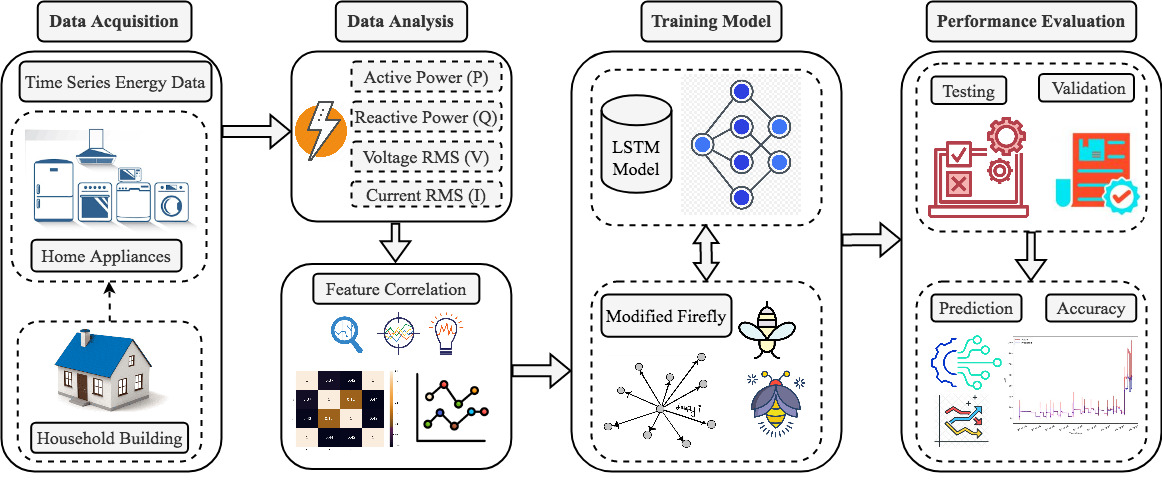
\includegraphics[height=2.92in]{energy prediction/Proposed model(11).jpg}
    \caption{The proposed scheme.}
    \label{fig:proposed model}
\end{figure*}


 
\section{Proposed Methodology} \label{Proposed Methodology}
This section explains the methodology of the proposed scheme, providing a detailed description of its related workflow. In this study, we introduce a novel hybrid model that combines LSTM and MFF to control energy consumption patterns over time. Figure \ref{fig:proposed model} illustrates the proposed model that comprises of different phases, including data acquisition, data analysis, training model, and performance evaluation.  

\subsection{Data Acquisition}
The data acquisition process is given in this section. The Portuguese home dataset is chosen because it contains important metrics and extensive time-series data on energy usage, which makes it ideal for accurate forecasting. This dataset is actively utilized in the state-of-the-art work and is openly available on the Open Source Foundation (OSF) repository, in contrast to other datasets that might have limited number of elements or restricted access. Table \ref{tab:appliances} gives a list of appliances ranging from kitchen appliances to electronic devices, which represents  high-dimensionality and nonlinear relationship in the dataset. The broad spectrum of appliances highlights the model's ability to capture a wide range of energy consumption behaviors, in order to adapt different household environments. 

\subsection{Data Analysis}
In this phase, the time-series data were extracted from the appliances and normalized. The extracted energy consumption features from the acquired dataset were in the form of active power, reactive power, voltage, and current. These features were analyzed using correlation coefficients to identify relationships between variables and complex patterns.
The data were further restructured using the sliding window technique to extract the sequential time-series data \cite{Ref2}. Sequential time-series data were provided as input to the training model step by step.

\subsection{Training Model}
To train the prediction model, all historical sequential inputs were fed to the LSTM model, an advanced variant of recurrent neural networks specifically designed to retain information over extended sequences and predict sequential data. During training, an LSTM model was initialized with hyperparameters as input, such as the number of hidden units, number of layers, sequence length, number of dense layers, and the learning rate. The number of hidden units and layers determines the model's complexity and capacity to capture non-linear and hierarchical patterns in the energy data, to balance between underfitting and overfitting. The sequence length controls the temporal range for learning dependencies, improving both prediction accuracy and computational efficiency. The learning rate plays a crucial role in ensuring stable and efficient model convergence during training. These hyper-parameters were fine tuned using a meta-heuristic MFF technique. The firefly in MFF technique generated a set of hyper-parameters in each iteration using a logistic chaotic map and further mapped them using a mapper function. The ModLSTM model iteratively learnt the consumption patterns from the training dataset and validated its prediction using the testing and validation dataset. The MSE was then calculated with respect to the test dataset, which was related to the corresponding firefly for the best fitness value. 

\subsection{Performance Evaluation}
Finally, the performance evaluation phase ensured the efficiency of the prediction model through a comprehensive comparative analysis with existing approaches. The model predictions were evaluated using testing and validation datasets to ensure reliability. Various evaluation metrics, including Root Mean Square Error (RMSE), Mean Absolute Error (MAE), Mean Absolute Percentage Error (MAPE), and $R^2$, were used to measure its accuracy and overall performance.  


 

\begin{table}[htbp]
\centering
\caption{List of appliances in the household building. }
\label{tab:appliances}
\begin{tabular}{|c|l|}
\hline
\rowcolor[HTML]{C0C0C0}
\textbf{ID} & \textbf{Appliance} \\ \hline
1 & Coffee Machine\\
\hline
2 & Fridge  \\
\hline
3 & Freezer \\
\hline
4 & Hand Mixer \\
\hline
5 & Hair Dryer + Straightener\\
\hline
6 & Kettle \\
\hline
7 & Macbook 2007 \\
\hline
8 & Macbook Pro 2011 (1) \\
\hline
9 & Macbook Pro 2011 (2) \\
\hline
10 & Microwave \\
\hline
11 & Stove + Oven \\
\hline
12 & TV Philips \\
\hline
13 & TV Sharp \\
\hline
14 & TV Grunding \\
\hline
15 & TV Samsung \\
\hline
16 & TV LG \\
\hline
17 & Toaster \\
\hline
18 & Vacuum Cleaner\\
\hline

\end{tabular}

\end{table}













\section{Mathematical Modeling}\label{Mathematical Modeling}
In this section, we discuss the overall mathematical framework for the proposed LSTM-MFF. The proposed model mainly consists of two components: LSTM for prediction and MFF for hyper-parameter optimization. In what follows, we present detailed information regarding these components.









\subsection{The LSTM Model}
The proposed scheme uses a DL-based framework that employs the LSTM model (see Fig. \ref{LSTM} for its architecture). The entire LSTM model consists of the following four fundamental components: forget gate, input gate, output gate, and cell state. These gates work together to handle the complex data, comprehend long-term dependencies, and account for the sequential features of the data. The model also has memory units that maintain state for a fairly long time. The training of this model is performed through input sequences from the dataset. Forget gate $f_t$ in an LSTM determines which information from the previous step should be retained during feed-forward propagation. This process is managed by initial activation function $\sigma$, as shown in Eq. \eqref{forget}.



\begin{figure}[!h]
    \centering
    \includegraphics[width= 9cm]{energy prediction/LSTM Architeture.drawio.png}
        \caption{Architecture of the LSTM approach.}
    \label{LSTM}
\end{figure}



 

\begin{equation}\label{forget}
f_t = \sigma \left( W_f \cdot [h_{t-1}, x_t] + b_f \right).
\end{equation}


In Eq. \eqref{forget}, the sigmoid activation function $\sigma$ calculates a value between 0 and 1 for each component of the cell state $C_{t-1}$, using the previous hidden state $h_{t-1}$ and the current input state $x_t$. This value is further applied through an element-wise multiplication operation on $f_t$ and $C_{t-1}$. Here, $b_f$ is a forget gate bias vector that modifies sigmoid activation function, providing greater flexibility and improving the model's learning efficiency. $W_f$ refers to forget gate weight matrix that measures how much information is retained or discarded. Specifically, a value of 1 preserves all information, while a value of 0 discards all information; the values between 0 and 1 control the proportion of information passed from previous state to current state (see Eq. \eqref{input}-\eqref{tanh input}).



\begin{equation}\label{input}
i_t = \sigma(W_i \cdot [h_{t-1}, x_t] + b_i)
\end{equation}
\begin{equation}\label{tanh input}
\tilde{C}_t = \tanh(W_c \cdot [h_{t-1}, x_t] + b_c)
\end{equation}
The next step includes selecting what information goes into the cell state. This is done in two stages. First, input gate $i_t$, which is a sigmoid layer, identifies the information that will be updated. Subsequently, a tanh layer computes a vector of new candidate values $\tilde{C}_t$, which could potentially be added in the cell state. These two values are integrated to update the cell state. The cell state acts as the memory in an LSTM, providing a major advantage over traditional recurrent neural networks for handling long sequences. At each time step, previous cell state $C_{t-1}$ interacts with the forget gate to determine what information should be retained. Furthermore, the updated information is combined with new inputs from input gate $f_t$ to create the new cell state $\tilde{C}_t$, or update memory (see in Eq. \eqref{cell state}).

   
\begin{equation}\label{cell state}
C_t = f_t \cdot C_{t-1} + i_t \cdot \tilde{C}_t
\end{equation}

Finally, the hidden state $h_t$ is calculated and passed through the softmax layer to produce its output $o_t$ after applying the hyperbolic tangent function ($tanh$) to the cell state $C_t$, as shown in Eq. \eqref{outut}-\eqref{tanho}. This essentially causes the cell state values to be scaled ranging from -1 to 1, which effectively filters their outputs. Next, the loss function, namely, Mean Squared Error (MSE),  calculates the difference between predicted output and actual target, providing a basis for error correction.




\begin{equation}\label{outut}
o_t = \sigma(W_o \cdot [h_{t-1}, x_t] + b_o)
\end{equation}



\begin{equation}\label{tanho}
h_t = o_t \cdot \tanh(C_t)
\end{equation}




\begin{equation} \label{Loss}
\text{Loss} = \frac{1}{N} \sum_{i=1}^{N} \left( y_i - \hat{y}_i \right)^2
\end{equation}

In the backpropagation process, gradients are propagated in the backward direction using loss as described in Eq. \eqref{Output gradient}-\eqref{candidate cell state gradient}. These gradients, $\frac{\partial Loss}{\partial o_t}$, $\frac{\partial Loss}{\partial C_t}$, $\frac{\partial Loss}{\partial f_t}$, $\frac{\partial Loss}{\partial i_t}$, $\frac{\partial Loss}{\partial \tilde{C}_t}$, are computed with respective gates, \textit{i.e.} $\hat{y}_t$, $h_t$, $f_t$, $i_t$, and $\tilde{C}_t$.


\begin{equation}\label{Output gradient}
    \frac{\partial Loss}{\partial o_t} = \frac{\partial Loss}{\partial h_t} \odot \tanh(C_t)
\end{equation}



\begin{equation}\label{cell state gradient}
    \frac{\partial Loss}{\partial C_t} = \frac{\partial Loss}{\partial h_t} \odot o_t \cdot (1 - \tanh^2(C_t)) + \frac{\partial Loss}{\partial C_{t+1}} \odot f_{t+1}
\end{equation}

\begin{equation}\label{forget gate gradient}
    \frac{\partial Loss}{\partial f_t} = \frac{\partial Loss}{\partial C_t} \odot C_{t-1}
\end{equation}

\begin{equation}\label{input gate gradient}
    \frac{\partial Loss}{\partial i_t} = \frac{\partial Loss}{\partial C_t} \odot \tilde{C}_t
\end{equation}


\begin{equation}\label{candidate cell state gradient}
    \frac{\partial Loss}{\partial \tilde{C}_t} = \frac{\partial Loss}{\partial C_t} \odot i_t \cdot (1 - \tanh^2(\tilde{C}_t))
\end{equation}

Furthermore, the weights and biases of each gate, \textit{i.e.} $W_f$, $W_i$, $W_c$, $W_o$, and $b_f$, $b_i$, $b_c$, $b_o$, are updated during the backpropagation process to minimize MSE. Finally, the weight and bias are updated using the standard method (see in Eq. \ref{weights update}-\ref{bais update}).

\begin{equation}\label{weights update}
\normalsize
    W_{t+1} = W_t - \eta \cdot \frac{\partial Loss}{\partial W_t}
\end{equation}


\begin{equation} \label{bais update}
\normalsize
    b_{t+1} = b_t - \eta \cdot \frac{\partial Loss}{\partial b_t}
\end{equation}



Next, the adjustment of weight and bias parameters is performed using the Adam optimizer by computing the gradients, such as $\frac{\partial Loss}{\partial W_t}$ and $\frac{\partial Loss}{\partial b_t}$ of the loss function with respect to these parameters. The current weight parameter $W_t$ and the current bias $b_t$ are adjusted in the direction that minimizes the loss function, \textit{i.e.} MSE, with the magnitude of updates specified by learning rate $\eta$. After each iteration $t$, the model has updated its weight  $W_{t+1}$  and bias $b_{t+1}$.

Similarly, the feed-forward and back-propagation processes are continued with each epoch. The model gradually learns by adjusting its parameters, which improves the prediction results over time. 


\begin{equation}\label{convergence}
\text{Stop training if } \frac{\text{Loss}_{\text{previous}} - \text{Loss}_{\text{current}}}{\text{Loss}_{\text{previous}}} < \epsilon
\end{equation}

Furthermore, the relative improvement between the previous loss value ${\text{Loss}_{\text{previous}}}$ and current loss value ${\text{Loss}_{\text{current}}}$ is calculated. The calculated loss indicates the reduction or enhancement in loss during each iteration. This process continues iteratively until the point when a model has minimized the error at the threshold $\epsilon$ and model is converged.







 

\begin{figure*}[!h]
    \centering
    \includegraphics[height=3in]{energy prediction/lstm-mffs.drawio(5).drawio.png}
    \caption{The process of hyper-parameter optimization using MFF.}
    \label{fig:A deep Learning Framework using LSTM and Modified Firefly}
\end{figure*}



\subsection{A Meta-heuristic Firefly Approach}

\subsubsection{The Conventional Firefly Approach}
The FF is a nature-inspired meta-heuristic approach. The primary purpose of the light behind these FF is to attract each other. The intensity of the fireflies decreases with distance, and fireflies move in search space for exploration. This nature-inspired behavior of fireflies is adopted by standard meta heuristic FF optimization, to optimize the solution. The FF approach operates with the following three factors: the mutual attraction of fireflies; their brightness (which establishes how attractive they are in relation to each other's distance), and the search region of the optimization problem responsible for controlling their luminescence. 


The equation of FF is given by Eq. \eqref{eq:firefly1}.

\textcolor{red}{
\begin{equation}\label{eq:firefly1}
    \resizebox{0.85\columnwidth}{!}{$
    \mathbf{x}_i(t+1) = \mathbf{x}_i(t) + \beta_0 e^{-\gamma r^2} (\mathbf{x}_j - \mathbf{x}_i) + \alpha(t)\mathbf{\epsilon}
    $}
\end{equation}}


\begin{equation}
\normalsize
\mathbf{x}_i(t+1) = \mathbf{x}_i(t) + \beta_0 e^{-\gamma r^2} (\mathbf{x}_j - \mathbf{x}_i) + \alpha(t) \mathbf{\epsilon},
\label{eq:firefly}
\end{equation}


where ${x}_i(t+1)$ and ${x}_i(t)$ represent the new position of the $i^{th}$ firefly at the time $t$+1 and the current position of the $i^{th}$ firefly at the time $t$, respectively. Furthermore, symbol $\beta_0$ is the initial attractiveness constant, defining the base level of attraction between fireflies. The symbol $e^{-\gamma r^2}$  depicts how attractiveness decreases with distance. Symbol $\gamma$ is the coefficient for light absorption that determines the rate at which attractiveness fades with distance. Meanwhile, symbol $r$ is the distance between $i^{th}$ and $j^{th}$ fireflies, calculated as $||{x}_j - {x}_i||$. This indicates the direction and magnitude of attraction of $j^{th}$ firefly to $i^{th}$ firefly, which also causes their movement. Finally, $\alpha(t)$ and ${\epsilon}$ are scaling factors for random movement and random vectors to add stochasticity to movement, allowing the firefly to explore the search space.




\subsubsection{A Novel Modified Firefly Approach}

As discussed above, the conventional FF is a meta-heuristic optimization technique inspired by the tendency of fireflies to flash. This method has issues, such as premature convergence and limited global search or exploration. The FF method is modified with additional parameters to resolve these issues of standard FF and to identify both local and global optimum values. These parameters are chaotic maps (logistic and Gauss/mouse maps) and levy flights (see the discussion below). 

\paragraph{Logistic Chaotic Maps}
Logistic chaotic maps generate initial population of hyper-parameter settings for the LSTM model, ensuring exploration of the search space. The logistic maps show chaotic behavior for certain parameters as shown in Eq. \eqref{log}.

\textcolor{red}{
\begin{equation}\label{log}
    \resizebox{0.6\columnwidth}{!}{$x_{n+1} = r x_n (1 - x_n), \quad 0 \leq x \leq 1$}
\end{equation}}



\begin{equation}\label{log}
    x_{n+1} = r x_n (1 - x_n), \quad 0 \leq x \leq 1 \quad 
\end{equation}
where \(x_n\) is a value at the current iteration \(n\), \(x_n+1\) is a value at the next iteration \(n+1\), and \(r\) is a parameter between 0 and 1 that determines the behavior of a map. Parameter \(x_n\) is an initial solution, generated using this map, avoiding local minima, and finding a global optimum.




\paragraph{Gauss Maps}
The Gauss maps update attractiveness parameter $\beta$, while the optimization process ensures the linear and non-linear updates for better exploration and exploitation. The Gauss map is defined as shown in Eq. \eqref{fraq}. 



\begin{equation}
\label{fraq}
{\beta_{t+1}} = \frac{1}{\beta_t}{\mod(1)}
\end{equation}
\textcolor{red}{At each iteration, the next value of $\beta$, $\beta_{t+1}$ is computed as the reciprocal of the current value $\beta_t$, with the results reduced to modulus 1}. This process produces a sequences of values that randomly appear and show chaotic behavior, ensuring that $\beta$ evolves unpredictably between 0 and 1. This enhances exploration across a large range of values and reduces the risks that the optimization process converges prematurely.














\paragraph{Levy Flights}
Finally, the levy flights parameters
are used to move fireflies to brighter fireflies with a step length, following a levy distribution, and ensuring the balance between local exploitation and global exploration. The step length of levy flights is calculated as shown in Eq. \eqref{levy}.


\begin{equation}\label{levy}
    X_i \leftarrow X_i + \text{Levy}(X_j - X_i)
\end{equation}
Eq. \eqref{levy} represents the step length using levy flights that is used to update the solutions to provide global search.  For example, symbols \(X_i\) and \(X_j\) represent the candidate solution in the search space. If \(X_j\) has a better fitness value than \(X_i\), then the algorithm moves \(X_i\) closer to \(X_j\). This movement improves the chances of converging towards the global optimum by exploiting the better solution \(X_j\) while exploring the search space.








\subsubsection{A Modified Firefly-driven LSTM Approach}


            In this subsection, we discuss the novel study that implements MFF with the LSTM approach (see Fig. \ref{fig:A deep Learning Framework using LSTM and Modified Firefly}).
            The proposed algorithm \ref{alg:WF} is designed to optimize the hyper-parameters of LSTM (see Table \ref{Hyperparameters Values Of Schemes}). The hyper-parameters are the number of hidden units of each LSTM layer, the number of layers, the length of the sequence, and the learning rate for the Adam optimizer, all of which are tuned using MFF. The inputs specify a range for these hyper-parameters, while the outputs include the total number of iterations and the number of fireflies used in the proposed approach. However, the mapping function is the core output that relates the optimal solution ($X_{opt}$) to the real hyper-parameter values within the predefined ranges.
Initially, ($X_{opt}$) is set to infinity, while parameter $\eta$ is set to 0.4, indicating the initial optimization point with the goal of decreasing the error. The firefly population is initialized using values generated by a logistic chaotic map by creating a vector for each firefly (see Eq. \eqref{vector}).




\begin{algorithm}[htp]
		\SetAlgoLined
		\DontPrintSemicolon
		\KwIn{
			\begin{itemize}
				\item 
				Hyper-parameters range for: number of hidden units, number of layers, sequence length, number dense layer units, learning rate. 
				\item Population size for the search algorithm N, max\_iterations.
		\end{itemize}} 
		\KwOut{opt\_solution \tcp{\small Best solution found for the hyper-parameters.} }
		\textbf{Initialize}:
		\begin{itemize}
			\item  $y^* = \infty$, $\eta = 0.4$  \tcp{\small $y^*$ as the best solution.}
	
			\item  $\mathbf{X}_n=[\mathbf{x}_1,\mathbf{x}_2,\mathbf{x}_3,...,\mathbf{x}_N],
			\mathbf{x}_n =[x_1,x_2,x_3,x_4,x_5], x_i\in [0,1]$. \tcp{\small initial population using logistic chaotic map.}
		\end{itemize}
		\textbf{Define}:
		\begin{itemize}
			\item 
			$\mathbf{h}(\mathbf{x}_n)$ = mapper($\mathbf{x}_n$,parameters\_range).
			\item $\mathbf{D}(\mathbf{x}_n) =$ Dataset($\mathbf{x}_n$)
			\item $F(\mathbf{x}_n)$  = LSTM( $\mathbf{D}(\mathbf{x}_n)$ , $\mathbf{h}(\mathbf{x}_n)$ ).
 			\item $y_n(F(\mathbf{x}_n) ) = $ MSE($F(\mathbf{x}_n)$ , true values) \tcp{\small cost function.}
		\end{itemize}
		
		\While{$t<$ max\_iterations}
		{
				 $\alpha = \alpha_0 0.9^{t}$\;
				 update $\beta$ via chaotic map operator (Gauss map).\;
				 Evaluate the population solutions $\mathbf{y}=[y_1(\mathbf{x}_1),y_2(\mathbf{x}_2),...,y_N(\mathbf{x}_N)]$.
				 $y^* = \min( \min(\mathbf{y}), y^* )$.\; %\tcp{\small update best cost.} 
				
				 $\mathbf{x}^* =\mathrm{arg\,min}(y^*)$\tcp{\small update best solution.}
				
				 		\For{i=1:N}{
					 \For{j=1:N}
					{
						 \If{$I_j>I_i$}
						{
							Move $X_i$ to $X_j$ using Levy flight step length
						}
					}
				}
				
		 }
		opt\_solution = mapper($\mathbf{x}^* $,parameters\_range)\;
		return opt\_solution 
		\caption{\centering The proposed LSTM-MFF-based optimized solution}
		\label{alg:WF}
	\end{algorithm}







\begin{equation}\label{vector}
    \text{[} x_1,x_2,x_3,x_4 \text{]},    \quad 0 \leq x_i \leq 1 \quad 
\end{equation}

Each $[x_i]$ given in Eq. \eqref{vector} is between 0 and 1. These vectors represent a potential solution corresponding to a set of LSTM hyperparameters. In addition, the fitness of each firefly is indicated as $F(X_n)$, which is calculated based on the MSE between the result predicted by the LSTM model trained using parameters derived from $X_n$ and the actual result in the test data set. The algorithm iteratively adjusts light absorption coefficient $\alpha$ using an exponential decay factor of 0.9. This reduces visibility of the fireflies to enhance exploitation capabilities. In addition, the attractiveness of fireflies $\beta$ is dynamically updated using a chaotic map, such as Gauss map. This helps to maintain diversity in the population and prevent premature convergence. During each iteration, the fitness value for each firefly is evaluated, and the best solution ($X_{opt}$) is updated. For instance, if a $j^{th}$ FF has a lower MSE than a firefly \textit{i}, then the algorithm moves the firefly from \textit{i} to \textit{j} using the Levy flight step length, thereby enabling both local and global exploration of hyper-parameter space. The iteration process continues until the maximum number of iterations is reached, ensuring a potential optimal setting for the LSTM hyperparameters.
       



\begin{table}[!h]
\centering
\caption{\centering Best hyper-parameter values achieved for the optimized prediction outcomes.}

\label{Hyperparameters Values Of Schemes}

\begin{tabular}{|p{0.22\linewidth}|p{0.1\linewidth}|p{0.12\linewidth}|p{0.12\linewidth}|p{0.12\linewidth}|}
\hline
\rowcolor[HTML]{C0C0C0}
\hline
\centering \textbf{Schemes} & \centering \textbf{Units} & \centering \textbf{N\_Layer} &  \centering\textbf{Sequence} & \textbf{L\_Rate }\\
\hline
Modified Firefly & \centering 72 & \centering 1 & \centering 23 & 0.010 \\
\hline
\centering Firefly & \centering 92 & \centering 1 & \centering 30 & 0.004 \\
\hline
\centering LSTM & \centering 15& \centering 1 & \centering 7 & 0.001 \\
\hline

\end{tabular}
\end{table}   










\section{Results and Discussion} \label{Results and Discussion}

In this section, we provide a comprehensive discussion on the simulation environment, a detailed analysis of the proposed scheme's findings, and compare the results with the existing schemes.

\subsection{The Simulation Environment}

The simulation environment used in the present study was set up with the following specifications: This includes a 12\textsuperscript{th} generation Intel(R) Core(TM), i9-12900 processor operating at 2400 MHz with 16 cores and 24 logical processors, supported by 32GB of RAM and a GeForce RTX 3080 GPU. The scheme development was performed on integrating the Spyder IDE, Keras, Scikit-learn, and TensorFlow 2.10 libraries with Python (version 3.9). In addition, MFF technique was designed independently, since it was not included in the built-in features of Niapy library used to implement nature-inspired algorithms.



\subsection{Data}

In this study, we used time-series energy data collected from various appliances within a Portuguese household over a period of 96 days (see Table \ref{tab:appliances} for further detail) \cite{Ref2}. The original dataset with one sample per second was preprocessed using the moving average. Next, one percent of the overall sample dataset was selected for the subsequent model implementation.






\begin{table}[htp]
\centering
\caption{Feature selection from the original dataset.}
\label{Features Selection of Time Series dataset}
\small
\begin{tabular}{|p{0.18\linewidth}|p{0.47\linewidth}|p{0.18\linewidth}|}
\hline
\rowcolor[HTML]{C0C0C0}
\textbf{Column} & \textbf{Description} & \textbf{Units} \\ \hline
Timestamp & Timestamp (YYYY-MM-DD-HH-MM-SS) when the record was collected (UTC) & \textit{Datetime}  \\
\hline
P & Active Power & \textit{Watt} \\
\hline
Q & Reactive Power & \textit{VAR}  \\
\hline
V & Voltage RMS & \textit{Volt}  \\
\hline
I & Current RMS & \textit{Amp} \\ \hline
\end{tabular}
\end{table}





\begin{table*}[htp]
  \centering
  \caption{Portuguese household dataset with timestamps.}
  \label{Dataset With Timestamps}
\resizebox{0.7\textwidth}{!}{
    \begin{tabular}{|c|c|c|c|c|}
    \rowcolor[HTML]{C0C0C0}
      \hline
      \textbf{Timestamp} & \textbf{P} & \textbf{Q} & \textbf{V} & \textbf{I} \\
      \hline
      2016-10-05  23:05:00:932 & 0.011932  & -0.006287 & 0.257812 & 0.027222 \\
      \hline
      2016-10-05 23:05:01.932 & 0.025208 & -0.013245  & 0.544525 & 0.057465 \\
      \hline
      2016-10-05 23:05:02.932 & 0.023010  & -0.012115 & 0.498199 & 0.052460 \\
      \hline
      2016-10-05 23:05:03.932 & 0.023285  & -0.012268 & 0.504639 & 0.053101 \\
      \hline
      2016-10-05 23:05:04.932 & 0.023834  & -0.012482 & 0.514771 & 0.054321 \\
      \hline
      ... & .... & .... & .... & .... \\
      \hline
      2016-12-31 16:11:52.343 & 0.083252  & -0.004486 & 0.490845 & 0.171295 \\
      \hline
      2016-12-31 16:11:53.343 & 0.086975  & -0.004730 & 0.512054 & 0.178833 \\
      \hline
      2016-12-31 16:11:54.343 & 0.081451  & -0.004395 & 0.479370 & 0.167450 \\
      \hline
      2016-12-31 16:11:55.343 & 0.088654  & -0.004791 & 0.521820 & 0.182220 \\
      \hline
      2016-12-31 16:11:56.343 & 0.000000  & 0.000000 & 0.000000 & 0.000000 \\
      \hline
    \end{tabular}%
  }
\end{table*}


\begin{table*}[htp]
  \centering
  \caption{Portuguese household dataset with timestamps.}
  \label{Dataset With Timestamps}
  \resizebox{0.7\textwidth}{!}{%   % reduced width to 70% of text width
    \begin{tabular}{|c|c|c|c|c|c|c|}
    \rowcolor[HTML]{C0C0C0}
    \hline
     \textbf{P} & \textbf{Q} & \textbf{V} & \textbf{I} & \textbf{MoH} & \textbf{DoW} & \textbf{HoD}\\
    \hline
    0.011932  & -0.0062873 & 0.257812 & 0.027222 & 5 & 2 & 23 \\
    \hline
    0.025208 & -0.013245 & 0.544525 & 0.057465 & 5 &  2 & 23 \\
    \hline
     0.023010 & -0.012115 & 0.498199 & 0.052460 & 5 & 2 & 23 \\
    \hline
    0.023285  & -0.012268 & 0.504639 & 0.053101 & 5 & 2 & 23 \\
    \hline
    0.023834 &  -0.012482 & 0.514771 & 0.054321 & 5 & 2 & 23 \\
    \hline
  \end{tabular}%
  }
\end{table*}



 
\begin{figure}[!h]
    \centering
    \includegraphics[width= 7cm]{energy prediction/newdata/corr_mat1s.png}
        \caption{Visualization of feature correlation of the data set.}
    \label{Features correlation }
\end{figure}
The dataset consisted of the following four features: active power ($P$), reactive power ($Q$), voltage ($V$), and current ($I$) normalized with suitable parameters (see Tables \ref{Features Selection of Time Series dataset}-\ref{Dataset With Timestamps}). The correlation analysis for these features showed a strong correlation between $P$ and $I$, indicating potential redundancy (see Fig. \ref{Features correlation }). Therefore, column $I$ was eliminated to reduce the complexity of the model. Concurrently, Minute of Hour (MoH), Day of Week (DoW), and Hour of the Day (HoD) were extracted from the original dataset (see Table \ref{Feature Extraction}). Thereafter, the dataset was divided into 80\% for training and validation (with 30\% of this used for validation) and  20\% for testing, resulting in the overall split of 56\% training, 24\% validation, and 20\% testing. 








\subsection{Evaluation Metrics}
The proposed scheme's performance was evaluated based on actual and predicted results. For the evaluations, different metrics were included. These metrics were RMSE, MAE, and MAPE, and $R^2$ error. Furthermore, average errors in a grouping of forecasts were determined by MAE, while the percentages of error per estimate were determined by MAPE. For evaluating the goodness of fit of a regression model, the metric $R^2$ is an effective approach. All such metrics are mathematically represented in Eq. \eqref{RMSE1}-\eqref{R_Score}.






 



\begin{equation}
RMSE = \sqrt{\frac{1}{n} \sum_{i=1}^{n} (\hat{y}_i - y_i)^2}.
\label{RMSE1}
\end{equation}


\begin{equation}
    MAE = \frac{1}{n} \sum_{i=1}^{n} \left| \hat{y}_i - y_i \right|.
    \label{MAE1}
\end{equation}


\begin{equation}
MAPE = \frac{1}{n} \sum_{i=1}^{n} \left| \frac{y_i - \hat{y}_i}{y_i} \right|.
\label{MAPE1}
\end{equation}


\begin{equation}
    R^2 = 1-\frac{\sum_{i=1}^{n} (y_i -\hat{y}_i^2)}{\sum_{i=1}^{n} (y_i- \bar{y}^2)}.
    \label{R_Score}
\end{equation}

where \(\hat{y}_i \), \( y_i \), and \( n \) represent predicted value, actual value, and the total number of observations, respectively. 



 \begin{figure}[!h]
		\centering
        \includegraphics[width=3in]{energy prediction/results_updated/Conv_eval_comparison1s.eps}
		\caption{\centering RMSE for the best firefly solution in each iteration using convergence graph.}
		\label{ff and mff}
	\end{figure}



 \begin{figure}[!h]
		\centering
		\includegraphics[width=3.55in]{energy prediction/results_updated/bar_plot_1sMAE.eps}
		\caption{\centering Comparison for the MAE using different algorithms.}
		\label{MAE}
	\end{figure}
\begin{figure}[!h]
		\centering
		\includegraphics[width=3in]{energy prediction/results_updated/bar_plot_1sRMSE.eps}
		\caption{Comparison for the RMSE using different algorithms.}
		\label{RMSE}
	\end{figure}

 	

  	\begin{figure}[!h]
		\centering
		\includegraphics[width=3in]{energy prediction/results_updated/bar_plot_1sMAPE.eps}
		\caption{Comparison for the MAPE using different algorithms.}
		\label{MAPE}
	\end{figure}

\begin{figure}[!h]
		\centering
		\includegraphics[width=3in]{energy prediction/results_updated/bar_plot_1sr2_score.eps}
		\caption{Comparison for the $R^2$ using different algorithms.}
		\label{R2}
	\end{figure}

 \begin{figure*}[!h]
	\centering
	\includegraphics[width=\linewidth, height=\linewidth]{energy prediction/newdata/PredictionsVsReal1s.png}
	\caption{\centering Visualization of the performance analysis of existing schemes and LSTM-MFF based on data variation.}
	\label{prediction vs real}
	%\vspace{-15pt}
\end{figure*}

\begin{figure*}[!h]
	%neeeds to be updated, xaxis -28:28
	\centering
	\includegraphics[scale=.56]{energy prediction/results_updated/scatter_plot_1s.png}
	\caption{An illustration of the proposed scheme vs. the existing schemes in terms of prediction of active power (in Watt).}
	\label{SCATTER PLOT}
	\vspace{-15pt}
\end{figure*}
\subsection{A Case Study of the Proposed Scheme}
As mentioned above, for a comprehensive analysis of the proposed ModLSTM model, the case study of energy consumption prediction at 1-second time interval was conducted. A key limitation of the standard FF lies in its initialization, which typically relies on uniform random sampling, leading to an unevenly distributed initial population. As a result, the algorithm's ability to explore the search space is restricted from the outset, increasing the risk of premature convergence. To address this challenge, this case study employs the MFF, where the population is strategically initialized using a logistic chaotic map. This approach ensures a more diverse and systematically distributed initial population, enhancing exploration and reducing convergence issues. Subsequently, LSTM was trained with a training dataset, and the parameters of LSTM were adjusted using a modified approach of fireflies in each iteration. Similarly, the best solution was updated at each iteration, and this process continued until it reached the convergence point. Fig. \ref{ff and mff} shows that the MFF converged after the sixth iteration, whereas FF converged after twelve iteration. It is observed that MFF provided broader coverage of the search space, preventing the model from stagnating at local minima and enhancing its ability to find superior solutions.







\subsection{Performance Comparison with the Existing Schemes }

The effectiveness of the proposed model was validated by comparing its performance with existing schemes, such as SVR, RFR, SAMFOR, LSTM, and LSTM-FF (see Fig. \ref{MAE}). Specifically, MAE was used to evaluate the performance algorithms, the lower value indicating a more accurate prediction. In the results, SVR and RFR showed the highest values of 55W and 32W, respectively, whereas SAMFOR's MAE amounted to 40W, which was higher than RFR, but lower than SVR. As compared to regression algorithms, LSTM showed extreme reduction in MAE, or 10W, while the LSTM-FF improved further, reducing MAE to 7W. Finally, the proposed LSTM-MFF showed the lowest MAE of 5W, indicating the most accurate prediction model in this comparison. 

Similarly, RMSE was measured to analyze the performance of aforementioned algorithms. The RMSE analysis in Fig. \ref{RMSE} showed that the traditional models, such as RFR, SVR and SAMFOR had a higher MAE value between 150W to 175W, indicating poor performance as compared to LSTM and LSTM-FF, which obtained 40W and 25W, respectively. However, the proposed LSTM-MFF model demonstrated the best performance among all algorithms in this analysis, with the lowest RMSE value of 20W. 
 Similarly, MAPE and $R^2$ were measured to evaluate prediction analysis of all algorithms (see Fig.\ref{MAPE} and \ref{R2}). Both plots showed that traditional models, such as RFR and SVR had the highest errors, with 6\% and 10\% MAPE, respectively, and 0.85 \(R^2\). Furthermore, the SAMFOR model had a MAPE of 5\% and 0.85 an \(R^2\), indicating unsatisfactory performance.
 However, LSTM achieved 0.9 $R^2$ and 3\% MAPE. Finally, LSTM-FF and LSTM-MFF both scored $R^2$ close to 1\% and 2\%, whereas MAPE values to 1\%. 
 In Addition, the comparative performance analysis also indicated that traditional models, such as RFR and SVR were effective for linear types of regression problems. These models faced issues to capture the non-linear and temporal dependencies of data. 
 Among the regression algorithms, the SAMFOR model performed better for predicting data with low variation; however, it significantly degraded the performance while applying high variation energy data. On the other hand, SVR and SAMFOR models also faced challenges dealing with the large datasets. Furthermore, the LSTM and LSTM-FF models captured long input sequences and temporal data; however, the LSTM-MFF technique fit the data more effectively, achieving reliable results. 
 
 
 Fig. \ref{prediction vs real} illustrates energy prediction for four-hour-ahead using various models, including RFR, SVR, SAMFOR, LSTM, LSTM-FF, and LSTM-MFF. The short-term variation caused mismatches in expected active power for both SVR and RFR, whereas SAMFOR model provided a slightly improved pattern assessing, but fell short in handling immense variations. The LSTM model generally outperformed other regression models, with the LSTM-FF improving response to fluctuations. As a result, the proposed LSTM-MFF closely matched the actual values in active power, particularly during impulsive power fluctuations.
 
   Fig. \ref{SCATTER PLOT} demonstrates that the proposed LSTM-MFF outperformed other algorithms. The SVR model significantly deviated from the optimum line, as actual values surpassed 1500 watts. Further, it predicted the higher actual values, with prediction data-points clustering below 1000 watts. RFR performed better; however, it still predicted under 1000 watts. The SAMFOR model indicated improvement, but its predictions for actual values above 2000 watts were still inadequate. On the other hand, the significant higher scattering was demonstrated in LSTM, especially for actual values above 1500 watts. To compare, the LSTM-MFF model showed a closed cluster of data points around optimum line, particularly for actual values above 2000 watts, where under-prediction was observed. Finally, the proposed LSTM-MFF aligned the most closely with the optimal line, effectively predicting both high and low values up to 3500 watts.

\begin{table}[!h]
    \centering
    \caption{\centering Comparison of the proposed solution with the existing schemes.}
    \label{Results per hour}
    \begin{tabular}{lcccc}
    \rowcolor[HTML]{C0C0C0}
        \hline
    \textbf{Schemes}  & \textbf{RMSE (W)} & \textbf{MAE (W)} & \textbf{MAPE} (\%) & \textbf{$R^2$ score}\\
        \hline
        SVR & 146.86 & 55.84 & 9.991 & 0.9200\\
        RFR & 142.76 & 35.60 & 5.696 & 0.9244 \\
        SAMFOR & 164.39 & 46.26 & 4.581 & 0.8997\\
        LSTM & 30.97 & 11.36 & 2.936 & 0.9964\\
        LSTM FF & 24.21 & 7.966 & 3.009 &0.9978\\
        LSTM-MFF & \textbf{23.554} & \textbf{6.605} & \textbf{2.512} &\textbf{0.9979}\\
        \hline
    \end{tabular}
\end{table}


The results of a comprehensive comparison of the proposed LSTM-MFF with existing schemes are shown in Table \ref{Results per hour}. In the table, the RMSE values for LSTM-FF and the proposed LSTM-MFF are very close, at 24.2 and 23.55, respectively. However, achieving this required additional processing time and iterations. MFF facilitated a faster identification of the optimal solution within the global search space, leading to earlier convergence. The computational efficiency of LSTM-MFF in terms of convergence stability and its superior prediction accuracy is also evaluated. Overall, the LSTM MFF obtained superior results as compared to the other schemes (namely, 23.554 RMSE, 6.605 MAE, 2.512 MAPE, and 0.9979 $R^2$). These results suggest that the proposed scheme accurately predicts irregular energy consumption with the highest precision.


\begin{figure}[!h]
		\centering
\includegraphics[width=3.5in]{boxplot.png}
		\caption{ \centering {ANOVA test to compare the performance of different algorithms.}}
		\label{Boxplot}
	\end{figure}


Further, the Analysis of Variance (ANOVA) test was implemented for statistical analysis to compare the performance of the different algorithms implemented in this study. The test was performed by first calculating the absolute error for each model that was previously defined as the difference between the predicted and actual values.  Subsequently, these errors distributions were analyzed using one-way ANOVA to assess statistical differences among the models. This test produced a p-value of 0, strongly rejecting the null hypothesis that all forecasting models have equivalent error distributions. 
Fig. \ref{Boxplot} shows the results of the ANOVA test using a boxplot and ensures that the differences in absolute errors among the models were statistically significant and not due to random variation. The box plot analysis revealed significant variations in the predictive performance of the models evaluated. SVR and RFR models demonstrated the highest median error of 19.43 and the broadest Interquartile Range (IQR), indicating inferior performance. Similarly, the SAMFOR model was performed comparably to the LSTM based approaches, and it attained second-lowest median error. LSTM and LSTM-FF obtained relatively lower median errors. The proposed ModLSTM model achieved the lowest median error of 3.07 and the tightest IQR between 1.43 and 5.70, which demonstrated superior accuracy compared to other approaches. The smaller IQR and lower whisker bounds of the proposed ModLSTM demonstrated its enhanced robustness and reduced variability in predictions.
 Overall, these results were aligned with performance evaluation metrics, particularly highlighting the superior accuracy of the LSTM variants and the proposed ModLSTM with the lowest error.











\begin{table*}
\centering
\caption{Energy prediction and optimization techniques} \label{tab:combined_comparison}
\begin{tabular}{|p{4.5cm}|p{5.2cm}|p{5.2cm}|}
\hline
\multicolumn{1}{c|}{\textbf{Approach}} & \multicolumn{1}{c|}{\textbf{Characteristics}} & \multicolumn{1}{c|}{\textbf{Limitations/ Gaps}} \\ \hline

SARIMA \cite{Ref40} & Better predictor than ARIMA in capturing linear and seasonal time series data. & Poor handling of highly non-linear data. \\ \hline

Linear SVR \cite{Ref44} & Efficient with small data sets. & Slower in dealing with huge data sets. \\ \hline

Nonlinear SVR with Gaussian kernel function \cite{Ref301} & Transforms non-linear data into linear form using kernel function. & Requires careful choice of kernel function. \\ \hline

LSSVR \cite{Ref47} & Improved efficiency in non-linear energy data sets. & Easily solves linear equations, but uses squared loss function. \\ \hline

RFR \cite{ref6} & Solves high-dimensional data, trains model faster. & Performs effectively only in short-term predictions. \\ \hline

LSTM \cite{Ref45} & Captures sequential and long-term dependencies, complex, nonlinear, time series data. & Slower and complex. \\ \hline

FF optimization technique \cite{Ref25} & Handles subdivisions, addresses multiple nodes, and simple design  & Issues to stuck at local minima due to exploration and exploitation. \\ \hline

Hybrid SAMFOR model \cite{ref4} & Strong capability for non-linear fitting. & Sensitivity to parameter tuning \\ \hline

PSO-optimized ANFIS2 hybrid \cite{RC59} & PSO tunes parameters to handle shifts in usage patterns; outperformed ANFIS, LSTM, and RF & PSO sensitivity to control parameters and search budget; ineffective in cross-domain generalization \\ \hline

DE-optimized deep architecture \cite{RC58} & DE searches optimal hyperparameters to improve prediction & Compute-intensive search\\ \hline

LSTM + meta-heuristic feature selection (Dragonfly, Firefly) \cite{RC57} & Dragonfly/Firefly algorithms select informative features to enhance LSTM forecasting & Study targets PV generation rather than whole-building load; performance depends on meta-heuristic parameterization  \\ \hline

PSO + LSTM hybrid \cite{RC56} & PSO tunes LSTM hyperparameters to improve short-term load forecasting & Focused on short-term horizons and converged prematurely  \\ \hline

Review of FA/PSO/DE in building energy analytics \cite{RC55} & Synthesizes Firefly, PSO, and DE in building energy prediction  & Issues such as local optima and parameter sensitivity in meta-heuristics \\ \hline







\end{tabular}
\end{table*}






\section{Conclusion} \label{Conclusion}
In this paper, we presented an effective DL framework for accurately forecasting building energy consumption. This framework contributes to achieving NZEB's goals for self-sustainability. The results revealed that the proposed ModLSTM framework achieved superior performance in capturing complex long-term dependencies and overcoming the limitations of existing schemes by amalgamating LSTM and MFF. The effectiveness of the proposed model was then evaluated against traditional energy consumption prediction techniques, such as RFR, SVR, SAMFOR, LSTM, and LSTM-FF. The regression and SAMFOR techniques handled low variation data, whereas LSTM and its extended techniques were found to achieve superior results with high variation data. Therefore, the energy prediction during 1-second time intervals highlighted the efficient outcome of the LSTM-MFF approach that converged faster, iterated less, and achieved the lowest MSE. These results offer important implications in the context of NZEBs initiatives, energy efficiency, and environmental sustainability. Further research can explore various areas of the applications of this framework in sustainable building practices. 

 \section*{Acknowledgements} This research was supported by the Department of Science and Technology (DST) and the India-Canada Centre for Innovative Multidisciplinary Partnerships to Accelerate Community Transformation and Sustainability (IC-IMPACTS), and the Centre of Excellence with grant NO. (DST/IC/IC-IMPACTS/2022/P-8 (G)).
 
 
 

\ifCLASSOPTIONcaptionsoff
  \newpage
\fi
\medskip
\bibliography{biblographyfile}
\bibliographystyle{ieeetr}
%\printbibliography
\end{document}





